\documentclass{article}
\usepackage{tikz, comment}
\usepackage{pifont}
\usepackage{fontspec, pgfplots}
\usetikzlibrary{arrows, decorations.markings, decorations.pathreplacing}
\begin{comment}
:Title: Not defined yet
:Tags: absolute value rules;properties of equality, equation rules;proper subset;equivalence properties of equality;set
:Prob: 0.7648;0.7631;0.66;0.6577;0.6125
:Author: Prof.Hu Ji-shan, HKUST
:Slug: No name yet

Description Here.........
\end{comment}
\begin{document}\centering 

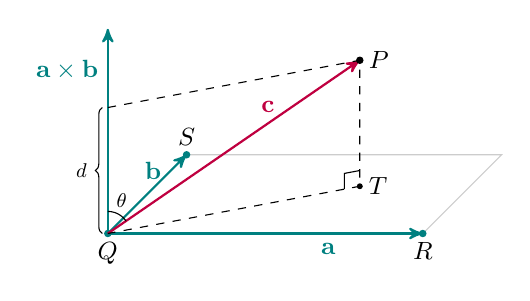
\begin{tikzpicture}[>=latex,xscale=.5*8, yscale=.5*8][font=\sf\small] 

\draw[teal, thick, ->, >=stealth'] (0,0)--(1, 0)
node[below, midway, pos=0.7, xshift=0, yshift=0, scale=1]{${\bf a}$};

\draw[teal, thick, ->, >=stealth'] (0,0)--(0.25, 0.25)
node[left, midway, pos=0.8, xshift=0, yshift=0, scale=1]{${\bf b}$};

\draw[teal, thick, ->, >=stealth'] (0,0)--(0, 0.65)
node[left, midway, pos=0.8, xshift=0, yshift=0, scale=1]{${\bf a} \times {\bf b}$};

\draw[gray!40] (0.25, 0.25)--++(1, 0)--++(-0.25, -0.25);

\draw[teal, fill] (0, 0) circle(0.01)node[black, below] {$Q$};
\draw[teal, fill] (1, 0) circle(0.01)node[black, below] {$R$};
\draw[teal, fill] (0.25, 0.25) circle(0.01)node[black, above] {$S$};

\draw[purple, thick, ->, >=stealth'] (0,0)--(0.8, 0.55)
node[left, midway, pos=0.7, xshift=0, yshift=2, scale=1]{${\bf c}$};

\draw[black, fill] (0.8, 0.55) circle(0.01)node[black, right] {$P$};

\draw[black, fill] (0.8, 0.15) circle(0.0075)node[black, right, scale=1] {$T$};

\draw[dashed] (0, 0.4) -- (0.8, 0.55)--++(0, -0.4)--(0,0);

\draw [decoration={brace,raise=2},decorate, xshift=0, yshift=0] 
(0,0)--(0, 0.4)node[black, left, midway, pos=0.5, xshift=-5, yshift=0, scale=0.8]{$d$};

\draw ({0.8+0.05*cos(-169.38)}, {0.15+0.05*sin(-169.38)}) --++(0, 0.05) -- ({0.8+0.05*cos(90)}, {0.15+0.05*sin(90)});

\draw[samples=100, smooth, domain=34.5:90, variable=\x] 
		plot ({0.07*cos(\x)}, {0.07*sin(\x)}); 

\node[black, xshift=5, yshift=12, scale=0.8] at (0, 0) {$\theta$};

\end{tikzpicture}
\end{document}